\section{Corpus}

In this section, the different corpus used will be introduced.
Two types of corpus were analyzed in this study.
The ones used in the PAN @ CLEF 2016 campaign~\cite{pan16}, which contain reviews and articles written in English, Dutch and Greek and 3 other literary corpus contain excerpts of English (1 corpus) and French (2 corpus) novels.

\subsection{Literature corpus}
\label{sec:lit_corpus}

Table~\ref{tab:lit_datasets} show corpus informations and statistics on the datasets.
These dataset contain large texts with 10'000 tokens in averages.
The number of text per authors relatively large, these dataset have a low $r$ value.

The corpus Oxquarry contain 52 excerpts from English novels from 9 different authors (Butler, Chesterton, Conrad, Forster, Hardy, Morris, Orczy, Tressel, Stevenson).
The dataset Oxquarry is already tokenized, which means every each words are on a seperated line.

The Brunet french corpus contain exactly 4 excerpts of novels for each of the 11 authors for a total of 44 excerpts.
Authors present in this dataset : Balzac, Chateaubriand, Flaubert, Marivaux, Maupassant, Proust, Rousseau, Sand, Vernes, Voltaire, Zola.
Brunet is already tokenized in two different ways : One using the actual tokens in the text, and another one using only the lemma.

St-Jean dataset was also used \cite{unine_corpus}.
It contains 200 excepts of french novels from 30 different authors.
Since this dataset is larger than the other one and was created such that it can be splited in two parts, the statistics of the two parts and the whole corpus is displayed in~\ref{tab:lit_datasets}.
One contain the first 100 texts and the other one the 100 following, which are called St Jean Serie A and St-Jean Serie B.
Both parts are approximatively containing the same number of authors and the same number of true links.

\begin{table*}[t]
  \caption{General information and statistics on the literary datasets}
  \label{tab:lit_datasets}
  \begin{tabular}{|l|l|l|l|l|l|l|l|l|}
    \hline
    \textbf{Name} &
    \textbf{Language} &
    \textbf{Authors} &
    \textbf{Texts} &
    \textbf{r} &
    \textbf{True links} &
    \textbf{Links} &
    \textbf{True links ratio} &
    \textbf{avg length} \\ \hline
    Oxquarry & EN & 9 & 52 & 0.173 & 160 & 1326 & 0.121 & 11650 \\ \hline
    Brunet & FR & 11 & 44 & 0.25 & 66 & 946 & 0.07 & 9778 \\ \hline
    St-Jean & FR & 30 & 200 & 0.15 & 670 & 19900 & 0.034 & 11533 \\ \hline
    St-Jean A 001-100 & FR & 17 & 100 & 0.17 & 330 & 4950 & 0.067 & 11552 \\ \hline
    St-Jean B 101-200 & FR & 19 & 100 & 0.19 & 258 & 4950 & 0.052 & 11513 \\ \hline
  \end{tabular}
\end{table*}


\subsection{PAN @ CLEF 2016}

During PAN @ CLEF 2016 clustering campaign which surveyed 8 submisssions, multiple dataset where given to the participents.
The dataset was splitted in two parts : a training part where 18 clustering problems and solutions was available and a second part with 18 problems the problems without solutions.
The problems are in 3 languages (English, Dutch, Greek) and two genres (articles and reviews) \cite{pan16}.

Detailled statistics on this dataset can be found in annex in Table~\ref{tab:pan_datasets}.
The r ratio is closer to 1 than 0 for most of the datasets, which indicate a rather larger number of single cluster.
Making the baseline \textit{Singleton Cluster} (each documents are considerd in a different cluster) a challanging problem to overcome for this dataset.
The mean size of these dataset is in the range $[171-1533]$ tokens, which can be considered as rather small datasets compared to the literary datasets presented in Section~\ref{sec:lit_corpus}.
Additionally the true links ratio is rather low for all problem which mean without strong comparaison metrics, finding the correct true links is even harder, thus Singleton Cluster better results in most of the cases.

\subsubsection{Text size importance in stylometry}

Figure~\ref{img:degradation} shows the importance of having texts large enough for a correct stylistic detection using distance between MFW vectors.

PAN16 dataset is a difficult dataset due to its small size, thus extracting reliable feature for each text to estimate each style is also a difficult task.
After multiple tests, the PAN @ CLEF 2016 dataset was not used in this study due to its difficulty in finding reliable stylographic clues.

\begin{figure}
  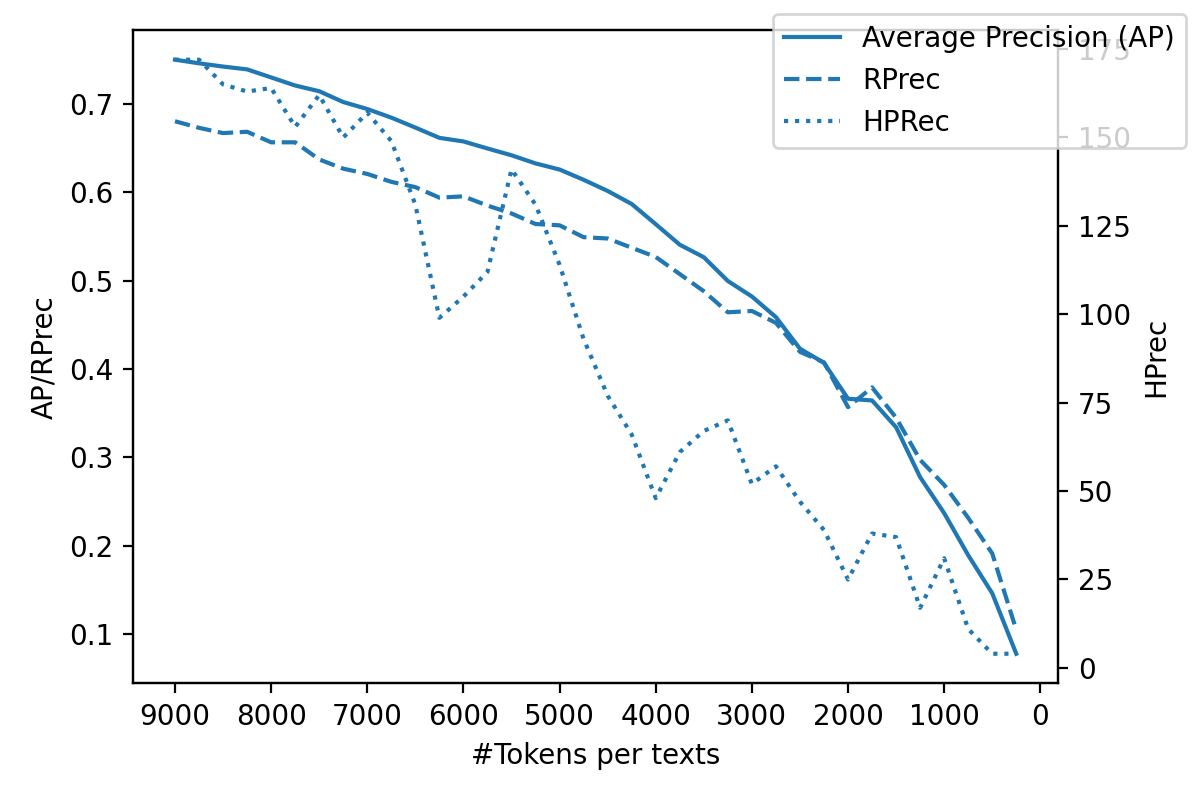
\includegraphics[width=\linewidth]{img/degradation.png}
  \caption{St-Jean ranks list evaluation on AP, RPrec and HPrec over the text size. Rank list computed using 500 MFW and the zscored-normalized cosine distance}
  \label{img:degradation}
\end{figure}
